\section{MUSIC-algoritmin simulointi}
Tässä kandidaattityössä käytettiin Matlab-ohjelmaa simuloimaan MUSIC-algoritmia ja sen eri versioita. Simulaatioita tehtiin yksinkertaisella pallomallilla sekä todellisten aivojen malleilla, jotka muodostettiin MRI-kuvantamisen avulla.



\subsection{MUSIC}
\begin{figure}[h]
    \centering
    \begin{minipage}{0.45\textwidth}
        \centering
        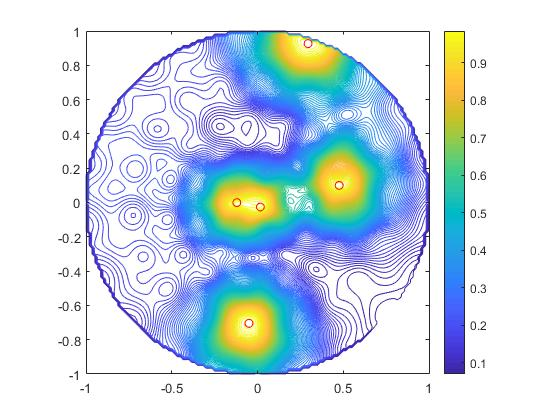
\includegraphics[width=1\textwidth]{MUSICfix.jpg}
    \end{minipage}\hfill
    \begin{minipage}{0.45\textwidth}
        \centering
        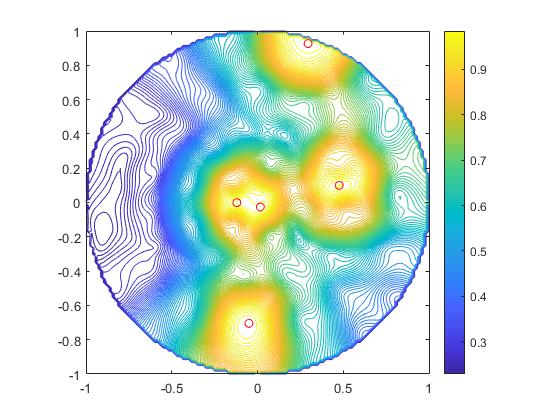
\includegraphics[width=1\textwidth]{MUSICfree.jpg} 
    \end{minipage}
    \caption{MUSIC-algoritmin simuloiminen pallomallin avulla Matlab-ohjelmalla. Punaiset pisteet ovat sattumanvaraisesti sijoitettuja lähteitä ja topografia on tehty MUSIC-algoritmin avulla. Vasemmanpuoleisessa kuvassa on skalaari-MUSIC ja oikeanpuoleisessa vektori-MUSIC. Molemmissa tapauksissa kohina on valkoista.}
    \label{fig:MUSIC}
\end{figure}

Kuvasta \ref{fig:MUSIC} huomataan, että MUSIC vapaalla orientaatiolla saa aikaan suuria aktiivisuuden alueita, mikä vaikeuttaa lähteiden paikantamista.

\clearpage
\subsection{RAP-MUSIC}
\begin{figure}[h]
    \centering
    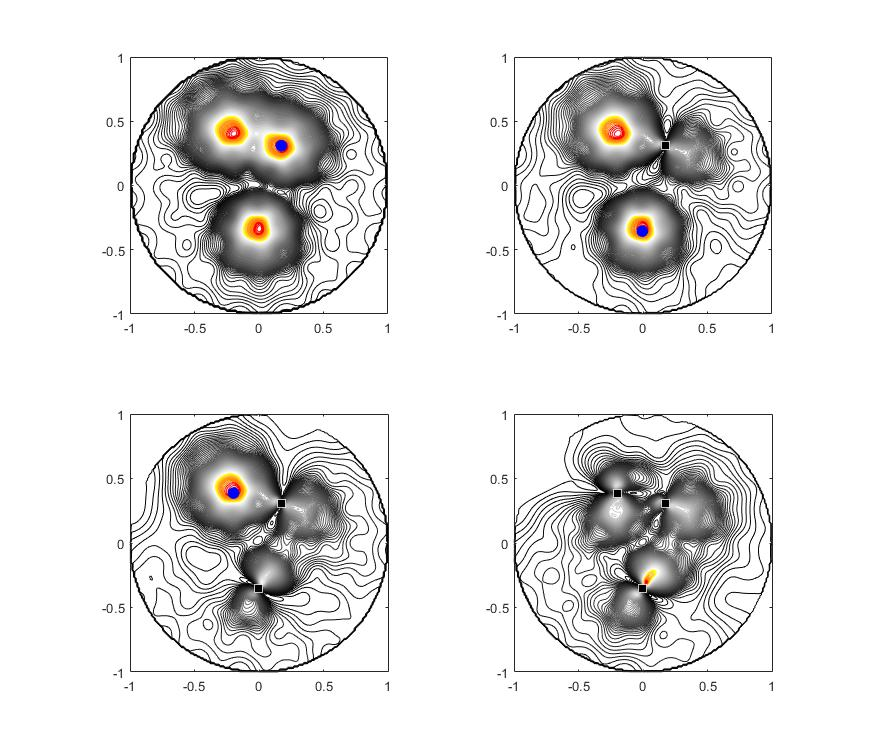
\includegraphics[width=1\textwidth]{rap11.jpg}
    \caption{RAP-MUSICin testausta pallomallilla ja kolmella lähteellä. Punainen väri kuvaa aktiivista aluetta. Algoritmin löytämä lähde on merkitty sinisellä ympyrällä ja löydetyt lähteet valkoreunaisella neliöllä}
    \label{fig:RAP}
\end{figure}

\subsubsection{TRAP-MUSIC}